\documentclass[a4paper, 10pt]{article}
    \usepackage[utf8]{inputenc}
    \usepackage{fullpage}
    \usepackage{enumitem}
    \usepackage{graphicx}
    \graphicspath{{images/}}
    \usepackage[urlcolor=blue]{hyperref}

    % No indent on new paragraph
    \setlength{\parindent}{0em}

    \setlength{\parskip}{1em}
    \renewcommand{\baselinestretch}{1.15}

    \title{COP 5615 - Project 2 Report}
    \author{Vaibhav Yenamandra ($1931$-$4050$)\\ email: \href{vyenaman@ufl.edu}{vyenaman@ufl.edu} }
    \date{\today}

    \begin{document}

    \maketitle

    \section{Gossip}
    From running times it is seen that the fastest topologies is one between Imperfect 2D grid and 2D grid, followed by the fully connected topology, then the line.
    \begin{figure}[h]
      \caption{Gossip Convergence Time v/s Network size}
      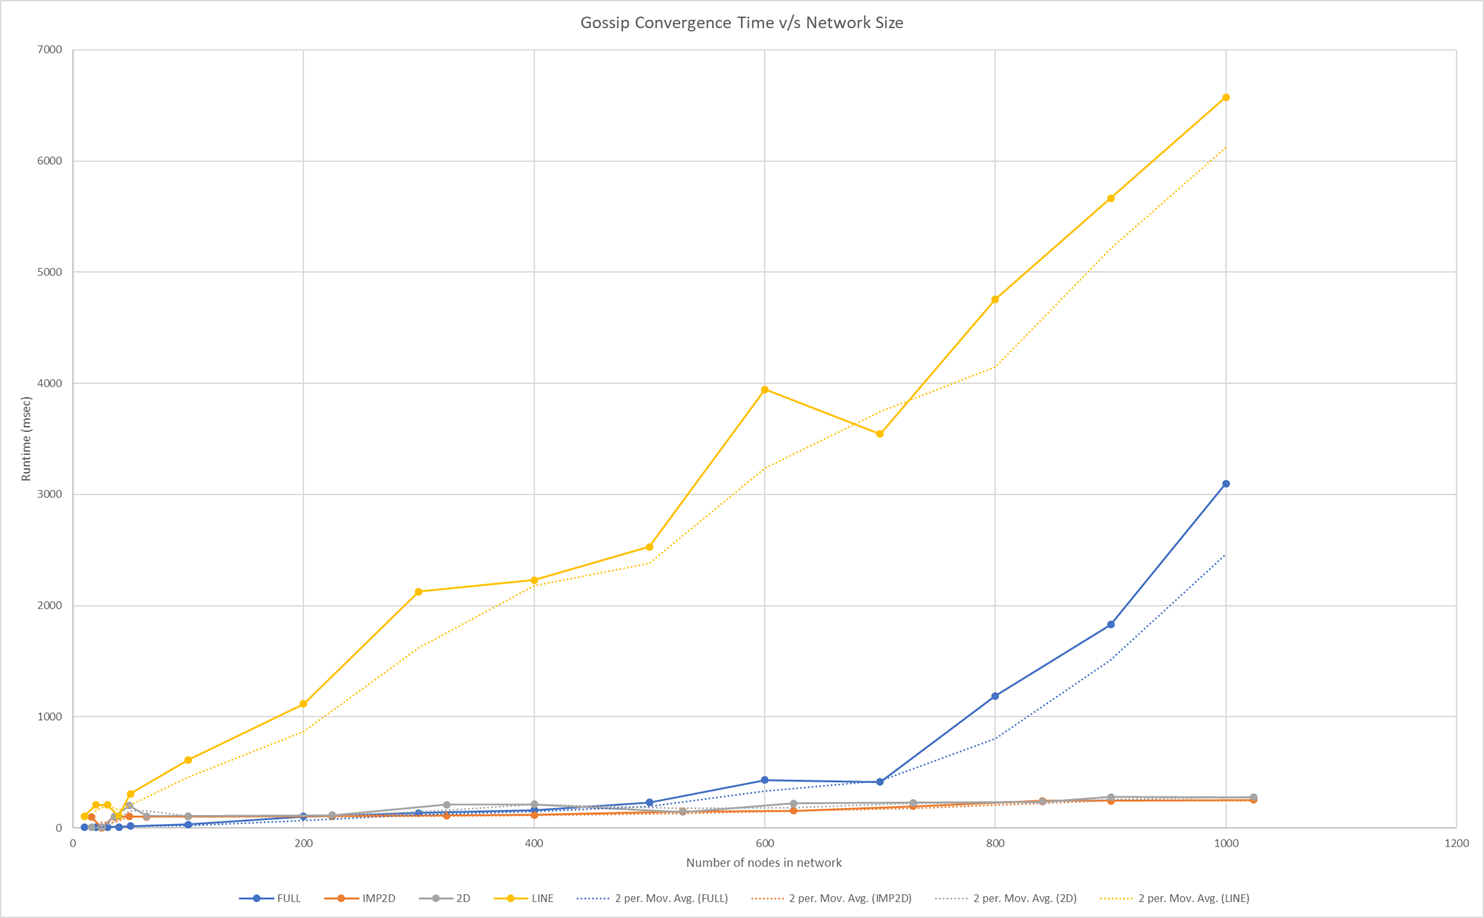
\includegraphics[width=\textwidth]{project2_gossip_chart}
    \end{figure}

    Covergence rates from the data extracted resemble the following:
    \begin{enumerate}
      \item{Line: $O(n)$}
      \item{Full: $O(n^2)$}
      \item{2D Grid: $O(\log n)$}
      \item{Imperfect 2D Grid: $O(\log n)$}
    \end{enumerate}

    The above figure shows the convergence times of various network topologies (see legend) vs the number of nodes in the network. For the project I defined convergence as the following routine:
    \begin{enumerate}
      \item{Check if more than $50\%$ of network is in a terminated state, if yes, return \texttt{true}, if not, go to the next step}
      \item{Check if less than $1\%$ of the network has not heard the rumour yet, if yes, return \texttt{true}, else return \texttt{false}}
    \end{enumerate}

    \section{Push-sum}
    While the graph for line may indicate that it converges to a suitable value very quickly, it is not to be trusted beyond networks of size 100-200 after which the variance among ``converged'' values is too high to be of any use.

    \begin{figure}[h]
      \caption{Push-sum Convergence Time v/s Network size}
      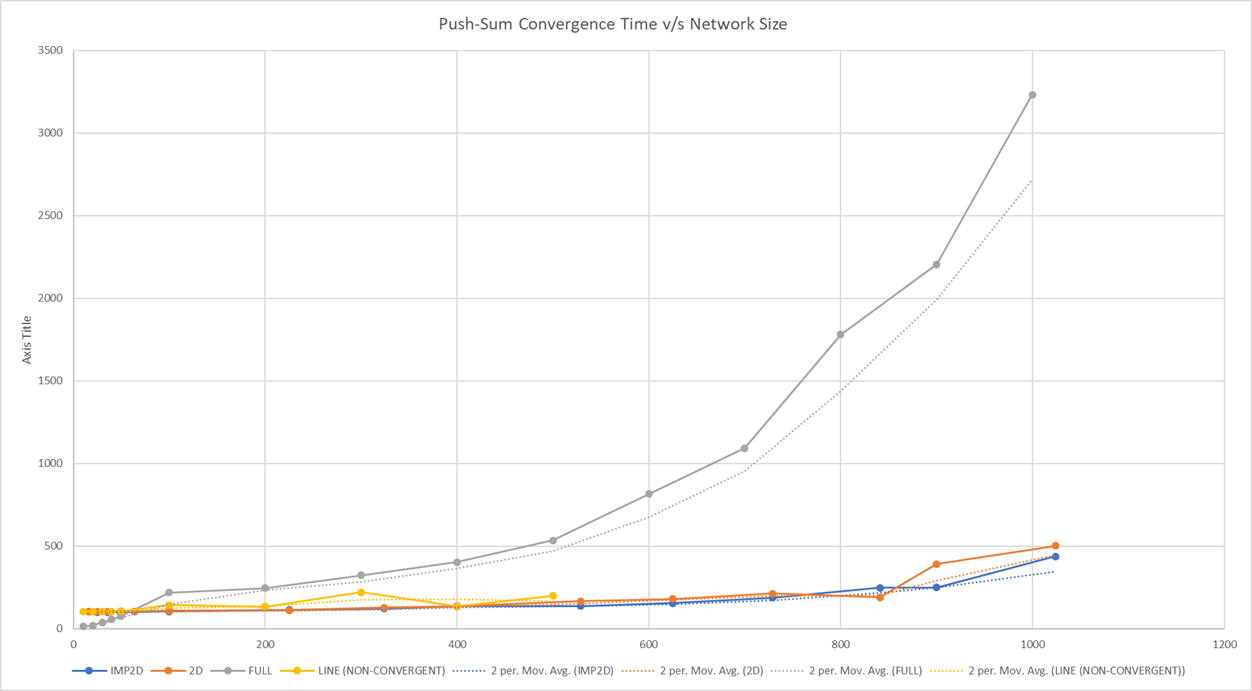
\includegraphics[width=\textwidth]{project2_psum_chart}
    \end{figure}

    Covergence rates from the data extracted resemble the following.
    \begin{enumerate}
      \item{Line: $O(n)$}
      \item{Full: $O(n^2)$}
      \item{2D Grid: $O(\log n)$}
      \item{Imperfect 2D Grid: $O(\log n)$}
    \end{enumerate}

    To check if the push sum network has converged we check if more than $50\%$ of the network has reached a stable value.

\end{document}
